\documentclass[11pt, a4paper]{article}
\usepackage{tikz}
\usepackage{amsmath}
\usepackage[dutch]{babel}
\usepackage[latin1]{inputenc} 
\usepackage{float}
\usepackage{calc}
\usepackage{algpseudocode}
\usepackage{algorithm}
\usepackage{textcomp}
\usepackage[T1]{fontenc}
\usepackage{lipsum}
\usepackage[skins]{tcolorbox}

\renewcommand{\algorithmicrequire}{\textbf{Input:}}
\renewcommand{\algorithmicensure}{\textbf{Output:}}

\newtheorem{opgave}{Opgave}

\begin{document}
	\title{Project Gretige Algoritmen}
	\author{Jarre Knockaert}
	\maketitle

\newpage

\section{Theoretische vragen}
\begin{opgave}
	Indien er 2 naburige toppen v en w een grote bedekking leveren, zal de top v met de hoogste graad worden toegevoegd aan de dominante verzameling en de buren zullen worden verwijderd. Het zou echter beter zijn om zowel v en w toe te voegen aan de dominante verzameling, want w leidt ook tot een hoge toename van de bedekking van de dominante verzameling. 
	Een voorbeeld van dergelijk geval, een graaf waarbij het algoritme zeer slecht presteert, zie je op figuur 1. Als we het algoritme uitvoeren op de graaf gebeurt het volgende:
	\begin{itemize}
		\item Neem top v = $4k+1$ met hoogste graad: $2k-1$. (Dit kon evengoed top $4k+2$ zijn, aangezien zijn graad gelijk is.)
		\item Voeg v toe aan de dominante lijst D. 
		\item Verwijder v en al zijn buren (top $1$ tot en met top $2k$) uit de graaf G. Nu bevat de G nog $2k-1$ toppen (top $2k+1$ tot en met top $4k$).
		\item De resterende toppen uit de graaf hebben elk graad 0 en zijn ge\"{i}soleerde toppen. (Aangezien hun enige buur werd verwijderd uit de graaf.) Voor elke top w van $2k+1$ tot en met top $4k$ gebeurt nu het volgende:
		\begin{itemize}
			\item Neem de top w. Aangezien elke top graad 0 heeft maakt het niet uit welke top we uit de graaf kiezen. Hun graad is (en blijft) gelijk aan elkaar. 
			\item Voeg w toe aan D. 
			\item Verwijder w uit G. De top w is geïsoleerd en dus er zullen ook geen extra toppen uit de graaf verwijderd worden. 
		\end{itemize}
	\end{itemize}
	In totaal werden $2k$ toppen toegevoegd aan de dominante lijst: top $4k+1$ en top $2k+1$ tot en met top $4k$. De minimale dominante verzameling bevat echter enkel de 2 toppen $4k+1$ en $4k+2$. 
	Het resultaat van het algoritme is een dominante verzameling met $\frac{2k}{2}=k$ keer meer toppen meer dan de optimale dominante verzameling. 
	\begin{figure}[H]
	%\centering
		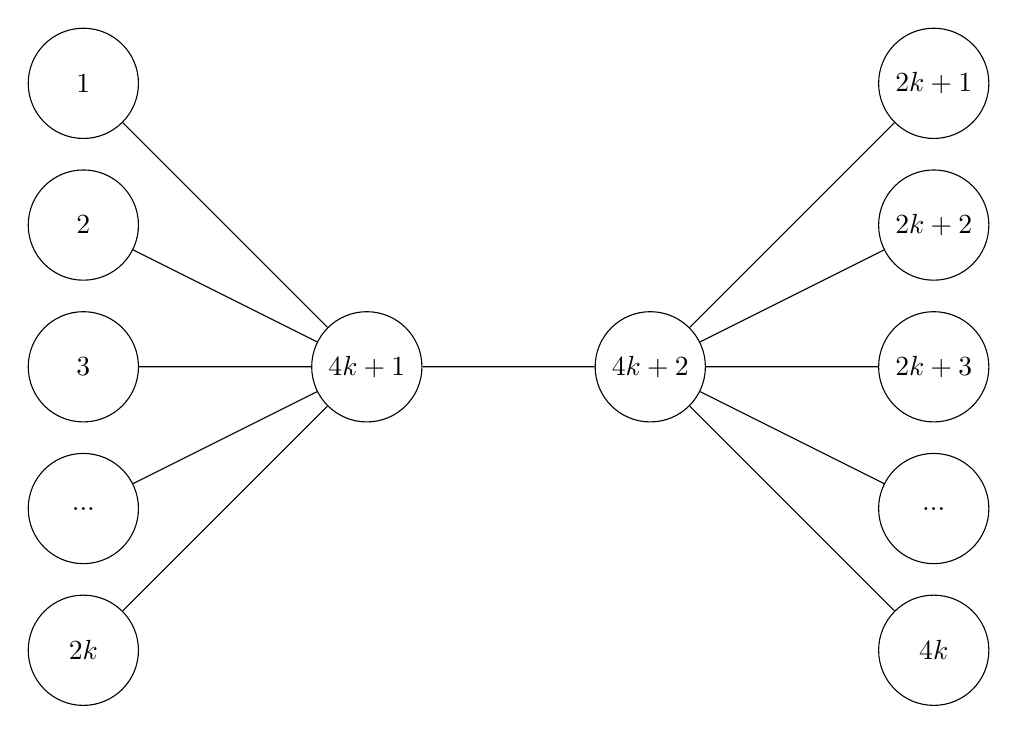
\begin{tikzpicture} 
		[main node/.style={circle, draw, minimum width=1.4cm, minimum height=1.4cm}, scale=1.8]
		\def\length{3}
			\foreach \a in {1,2,...,\length}{
				\node[main node]  (\a) at (0, 2+\length-\a) {$\a$};
				\node[main node]  (2k+\a) at (6, 2+\length-\a) {$2k+\a$};
			}
			\node[main node]  (leftdots) at (0, 1) {...};
			\node[main node]  (rightdots) at (6, 1) {...};
			\node[main node]  (2k) at (0, 0) {$2k$};
			\node[main node]  (4k) at (6, 0) {$4k$};
			\node[main node] (4k+1) at (2,2) {$4k+1$}; 
			\node[main node] (4k+2) at (4,2) {$4k+2$}; 
	
			\path (leftdots) edge node {} (4k+1);
			\path (rightdots) edge node {} (4k+2);
			\path (4k+1) edge node {} (4k+2);
			\path (2k) edge node {} (4k+1);
			\path (4k) edge node {} (4k+2);
			\foreach \a in {1,2,...,\length}{
				\path (\a) edge node {} (4k+1);
				\path (2k+\a) edge node {} (4k+2);
			}
		\end{tikzpicture}
		\caption{Een graaf waarbij het algoritme slecht presteert.}
	\end{figure}
\end{opgave}
\begin{opgave}
\end{opgave}
\begin{opgave}
	
		Hier volgt een uitvoerige bespreking van de algoritmes. 
		\begin{tcolorbox}[blanker,float=tbp, grow to left by=1cm,grow to right by=1cm]
		\begin{algorithm}[H]
			\caption{Dominante verzameling van vlakke grafen}
			\begin{algorithmic}[1]
				\Require Een planaire graaf G(V(G),E(G)
				\Ensure Een dominante verzameling D
				\State $totalCoverage \gets 0$
				\State Count-sort V(G) op basis van de graad van de toppen\label{sortoperation}
				\ForAll{$v\ |\ v \in V(G) \land deg(v)=1$}\Comment{Optimalisatie 1}\label{startoptimalizationloop1}
					\State Neem $w\ |\ wv \in E(G)$\Comment{v heeft \'{e}\'{e}n buur}
					\If{w nog niet bezocht $\land$ coverage(w) > 0}
						\State $D \gets D \cup \{w\}$
						\State bezoek w 
						\State $totalCoverage \gets totalCoverage+1$
						\State $coverage(w) \gets 0$
					\EndIf 
					\ForAll {$u\ |\ u \in V(G) \land uw \in E(G)$}
						\State $coverage(u) \gets coverage(u) - 1$
						\If{u niet bezocht}
							\State bezoek u
							\State $totalCoverage \gets totalCoverage + 1 $
						\EndIf
					\EndFor
					\If{$totalCoverage = |V(G)|$}
						\State Stop de foreach loop
					\EndIf 
				\EndFor\label{endoptimalizationloop1}
				\ForAll{ $minimum \in \{6, 5,...,0\}$} \Comment{Optimalisatie 2}\label{startoptimalizationloop2}
					\State $i \gets 0$
					\While{$starttotalCoverage < |V(G)| \land i<|V(G)|$}\label{startactualalgorithmloop}
						\State Neem v, de i-de top, $\in$ V(G)
						\If{coverage(v) > 0}
							\State Neem max | $(\forall u \in N_G(v)) \land (max \ne u) \Rightarrow coverage(max)>coverage(u))$\label{neighbourloop1}
							\If{coverage(v) > coverage(max)}
								\State max $\gets$ v
							\EndIf
							\If{coverage(max) > minimum}
								\State actualCoverage $\gets \{w\ |\ w \in N_G(max) \land w\ niet \  bezocht\}|$\label{neighbourloop2}
								\If{actualCoverage > minimum}
									\State totalCoverage $\gets$ totalCoverage + actualCoverage
									\State $coverage(max)  \gets 0$
									\State $ D \cup \{max\}$
									\State Bezoek max en zijn buren\label{neighbourloop3}
								\EndIf 
							\EndIf
						\EndIf
						\State $i \gets i+1$
					\EndWhile\label{endactualalgorithmloop}
				\EndFor\label{endoptimalizationloop2}
				
			\end{algorithmic}
		\end{algorithm}
		\end{tcolorbox}

		Enkele belangrijke vermeldingen bij algoritme 1. 
		\begin{itemize}
		\item Een buur is bezocht indien de top element is van de dominante verzameling of indien een buur van deze top element is van de dominante verzaleming.
		\item De bedekking/coverage van een top is de bovengrens van het aantal onbezochte buren.
		\item De werkelijke bedekking/coverage van een top is gelijk aan het aantal onbezochte buren. 
		\item De coverage van een verzameling van toppen is een som van de coverage van alle buren.
		\item De totalCoverage is de de som van de coverage van alle buren. Indien de coverage gelijk is aan |V(G)|, dan is de dominante verzameling klaar. 
		\item De variabele minimum stelt een ondergrens voor van de werkelijke coverage een top moet bieden aan de graaf voor de top kan toegevoegd worden aan de dominante verzameling.
		\end{itemize}
		
		Algoritme 1 loopt in lineaire tijd. Ik zal de verschillende delen van het algoritme bespreken om de complexiteit te verklaren. Beschouw bij deze analyse n als het aantal toppen. De lijnen die niet besproken worden zijn triviaal en hebben constante tijd $\Theta(1)$.
		\begin{itemize}
			 \item Lijn \ref{sortoperation}: Hier wordt counting sort toegepast op de toppenverzameling om deze te ordenen op basis van hun graad. De complexiteit van counting sort is O(n+k). Hier is k (de graad) begrensd door n-1. De totale complexiteit is hier $O(2n-1)$.
			 \item Lijn \ref{startoptimalizationloop1} $\rightarrow$ \ref{endoptimalizationloop1}: Er wordt ge\"{i}tereerd over de toppen met graad 1. Dit zijn er hoogstens n-1. Stel v de top met graad 1 en w de enige buur van deze top. 
			 Er wordt ge\"{i}tereerd over alle aanliggende bogen van w. Elke boog wordt hoogstens 2 keer bekeken. De reden hiervan is dat de top w maar \'{e}\'{e}n keer wordt genomen als naburige top van top v met graad 1. Er wordt eenmalig ge\"{i}tereerd over al zijn aanliggende bogen. De aanliggende bogen kunnen echter nogmaals \'{e}\'{e}n bekeken worden bij het itereren over de bogen van een buur van een andere top met graad 1. 
			 Elke boog kan dus hoogstens 2 keer bekeken worden bij het itereren over de bogen van toppen die een buur zijn van een top met graad 1. De boog van een top met graad 1 wordt ook maar twee keer bekeken, eens om zijn buur te bepalen, nogmaals tijdens het itereren over de bogen van zijn buur. In het geheel wordt dus elke boog hoogstens 2 keer bekeken. 
			 In een planaire graaf zijn er hoogstens $3n-6$ bogen. De volledige lus is dus lineair in het aantal toppen. De totale complexiteit is hier $O(2*(3n-6)) = O(6n-12)$
			\item Lijn \ref{startoptimalizationloop2}: De for lus wordt juist 6 keer uitgevoerd. De totale complexiteit is hier 
			$O(6*(complexiteit\ van\ elke\ iteratie))$
			\item Lijn \ref{startactualalgorithmloop} $\rightarrow$ \ref{endactualalgorithmloop} : De complexiteitsanalyse van deze lus is gelijkaardig aan de complexiteitsanalyse van lijn \ref{startoptimalizationloop1} $\rightarrow$ \ref{endoptimalizationloop1}. De buitenste lus gebeurt hoogstens n keer. (i stelt de index voor van de huidige top.) Eerst wordt lokaal gezocht naar het maximum via de aanliggende bogen van top v. Elke aanliggende boog wordt nu hoogstens \'{e}\'{e}n keer bekeken op lijn \ref{neighbourloop1}. Dit wordt hoogstens 1 keer uitgevoerd bij elke top, een boog heeft 2 eindpunten, dus wordt hoogstens 2 keer vanuit elk eindpunt bekeken. Vervolgens op lijn \ref{neighbourloop2} wordt opnieuw ge\"{i}tereerd over de bogen van de node max. Een node kan hoogstens \'{e}\'{e}n keer als max genomen worden. $n-2$ nodes kunnen als maximum gekozen worden. Elke boog kan op deze lijn opnieuw hoogstens 2 keer overlopen worden, 1 keer vanuit zijn beide eindpunten indien beide eindpunten eens de max node zijn. Als laatste wordt ook op lijn \ref{neighbourloop3} nogmaals over dezelfde bogen als op lijn \ref{neighbourloop2} ge\"{i}tereerd. Elke boog wordt op deze lijn dus ook hoogstens 2 keer bekeken. In totaal wordt deze boog dus hoogstens 4 keer bekeken. Nu kan dus elke boog hoogstens 6 keer bekeken worden in de volledige while-lus. In een planaire graaf zijn er hoogstens $3n-6$ bogen. De volledige lus is dus lineair in het aantal toppen. De totale complexiteit is hier $(O(6*(3n-6)))=O(18n-36)$.
		
		
		De volledige complexiteit is nu: 
		\[(2n-1)+(6n-12)+(18n-36)=26n-49\ (=O(n))\]
		
			Het algoritme is gretig aangezien we itereren over de toppen en telkens lokaal zoeken naar de best toe te voegen top. De top die het beste lijkt wordt vervolgens toegevoegd aan de lijst, en zo wordt ()het grootste deel van de) verzameling opgebouwd. Het algoritme is nu dus per definitie gretig aangezien het bij elk stadium naar het lokale optimum zoekt.
			Het gretig algoritme heeft 5 onderdelen: (De 5 onderdelen van een gretig algoritme volgens wikipedia.)
			\begin{itemize}
				\item Een kandidaatverzameling: de verzameling D
				\item Een selectie functie: het lokaal zoeken naar de optimale top
				\item Een haalbaarheidsfunctie het vergelijken van de eigenlijke bedekking van een top met 0. 
				\item Een objectieve functie: het toevoegen van het maximum aan de verzameling D
				\item Een oplossing functie: het vergelijken van de actualCoverage met |V(G)|
			\end{itemize} 
			 Vooraf worden ook toppen toegevoegd die buur zijn van een top met graad 1. Hier wordt niet gekeken naar de bedekking van de top. Het is een optimalisatie en wordt voorafgaand aan het werkelijk gretig algoritme uitgevoerd. 
		\end{itemize}
\end{opgave}
\section{Implementatie}
\subsection{Dominantie in vlakke grafen}
\end{document}